\chapter{INTRODUCTION}
\label{chap:introduction}

\section{Outline}
In an era where healthcare is becoming increasingly digital, the volume of patient data being generated each day has grown exponentially. However, this growth has not been matched by equivalent progress in data ownership, privacy, or interoperability. Medical records are typically stored within centralized databases managed by hospitals, clinics, and laboratories — systems that are often incompatible with each other and vulnerable to breaches. Patients rarely have visibility or control over their personal health information, and data-sharing between institutions remains inefficient and insecure.

To address these critical issues, MediVault has been conceptualized and developed as a blockchain-based healthcare data sharing system. It enables patients to securely store, manage, and share their encrypted medical data through a decentralized and transparent network. Beyond security, MediVault extends into the ethical realm by introducing an Anonymized Opt-in Research Module. This feature allows patients to voluntarily contribute de-identified medical data to research projects while maintaining full control over their consent — achieving a delicate balance between individual privacy and collective scientific progress. Built using Ethereum blockchain, Solidity smart contracts, Truffle, Ganache, Web3.js, and React.js, MediVault creates a fully decentralized ecosystem where every operation — from record creation to data sharing — is verified, recorded, and immutable.

\section{Problem Statement}
Traditional Electronic Health Record (EHR) systems rely on centralized architectures that introduce several issues. These include security vulnerabilities, unauthorized data access, duplication of medical records, and lack of transparency in data handling. Moreover, in many research scenarios, hospitals anonymize and sell patient data without explicit consent — raising ethical and legal concerns. MediVault addresses these problems by establishing a patient-centric data ownership model on the blockchain. Every piece of health information and every permission is governed by smart contracts, ensuring that data cannot be altered, deleted, or shared without patient approval. The system thereby restores autonomy to the patient while preserving data security and accountability.

The core problems with existing systems can be summarized as follows:
\begin{itemize}
    \item \textbf{Lack of Patient Control:} Patients have little to no control over who accesses their medical data. Once shared with a provider, the data is often stored in proprietary systems, making it difficult for patients to track its usage.
    \item \textbf{Data Silos:} Medical data is fragmented across various healthcare providers, leading to incomplete patient histories and diagnostic inefficiencies. Interoperability between different EHR systems is a persistent challenge.
    \item \textbf{Security Risks:} Centralized databases are prime targets for cyberattacks. A single breach can expose the sensitive health information of thousands of patients.
    \item \textbf{Inefficient Data Sharing:} Sharing data between providers is often a manual and slow process, involving faxes or insecure emails. This can delay critical medical treatments.
    \item \textbf{Ethical Concerns in Research:} The secondary use of patient data for research often occurs without the explicit and ongoing consent of the patient, raising significant ethical questions.
\end{itemize}

MediVault is designed to systematically address each of these challenges by re-architecting the health data ecosystem around the principles of decentralization, patient consent, and cryptographic security.

\section{Motivation}
The motivation behind MediVault arises from two key needs: patient empowerment — giving individuals direct control over their medical information — and ethical research enablement, which allows large-scale health data analysis while respecting personal privacy. The growing misuse of medical data, coupled with the necessity of data-driven healthcare innovation, demands a system that protects both privacy and progress. MediVault provides precisely this — a platform where patients become active participants, choosing when and how their data can be shared for research, and ensuring transparency through blockchain verification.

The project is driven by the vision of a healthcare system where technology serves the patient first. By leveraging the inherent properties of blockchain—immutability, transparency, and decentralization—we can build a new paradigm for health data management. This new paradigm shifts the balance of power from institutions to individuals, fostering a more collaborative and trustworthy relationship between patients, providers, and researchers. The potential to accelerate medical research by providing a secure and ethical platform for data sharing is another significant motivator.

\section{Purpose}
The purpose of MediVault is to design and develop a secure, decentralized healthcare data sharing platform that enables patient ownership and management of medical records, secure data exchange between patients, doctors, and researchers, end-to-end encryption and tamper-proof data storage using blockchain, and voluntary and revocable consent for anonymized research participation. By achieving these goals, MediVault envisions a healthcare ecosystem that is secure, ethical, transparent, and fundamentally patient-first.

The primary objectives of the project are:
\begin{enumerate}
    \item To implement a decentralized application (DApp) that allows patients to upload, view, and manage their health records.
    \item To develop Solidity smart contracts that govern data access, patient consent, and record sharing logic.
    \item To integrate MetaMask for secure user authentication and transaction signing.
    \item To create an Anonymized Opt-in Research Module that allows researchers to access de-identified data with patient consent.
    \item To ensure the confidentiality and integrity of health data through encryption and hashing mechanisms.
    \item To build a user-friendly interface using React.js that simplifies interaction with the blockchain.
\end{enumerate}

\section{Project Roadmap}
The development of MediVault followed a structured roadmap, divided into distinct phases to ensure a systematic and iterative development process. Each phase built upon the previous one, culminating in a fully functional prototype.

\tikzstyle{startstop} = [rectangle, rounded corners, minimum width=3cm, minimum height=1cm,text centered, draw=black, fill=red!30]
\tikzstyle{io} = [trapezium, trapezium left angle=70, trapezium right angle=110, minimum width=3cm, minimum height=1cm, text centered, draw=black, fill=blue!30]
\tikzstyle{process} = [rectangle, minimum width=3cm, minimum height=1cm, text centered, draw=black, fill=orange!30]
\tikzstyle{decision} = [diamond, minimum width=3cm, minimum height=1cm, text centered, draw=black, fill=green!30]
\tikzstyle{arrow} = [thick,->,>=stealth]

\begin{figure}[h!]
\centering
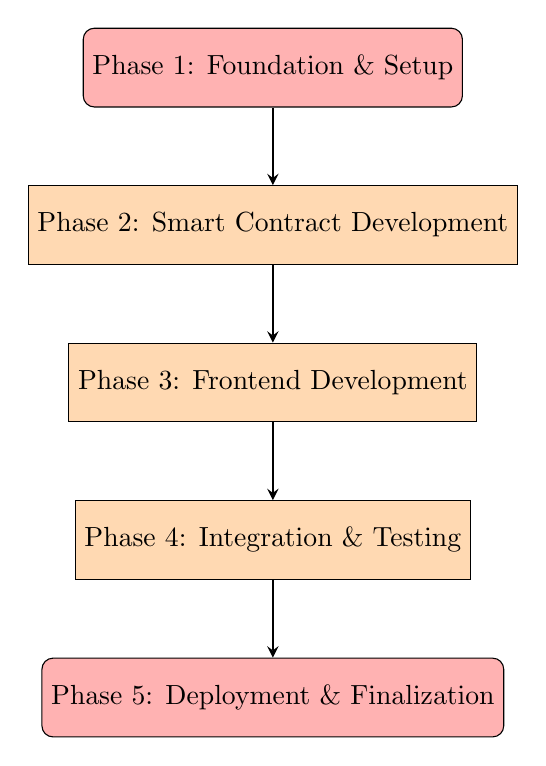
\begin{tikzpicture}[node distance=2cm]
\node (start) [startstop] {Phase 1: Foundation \& Setup};
\node (pro1) [process, below of=start] {Phase 2: Smart Contract Development};
\node (pro2) [process, below of=pro1] {Phase 3: Frontend Development};
\node (pro3) [process, below of=pro2] {Phase 4: Integration \& Testing};
\node (stop) [startstop, below of=pro3] {Phase 5: Deployment \& Finalization};

\draw [arrow] (start) -- (pro1);
\draw [arrow] (pro1) -- (pro2);
\draw [arrow] (pro2) -- (pro3);
\draw [arrow] (pro3) -- (stop);

\end{tikzpicture}
\caption{Project Development Phases}
\label{fig:roadmap}
\end{figure}

\subsection{Phase 1: Foundation and Environment Setup}
This initial phase focused on establishing the development environment and foundational technologies. Key activities included:
\begin{itemize}
    \item Setting up the Node.js environment and installing necessary packages.
    \item Installing and configuring the Truffle Suite for smart contract development.
    \item Setting up a local blockchain using Ganache for testing and deployment.
    \item Initializing the React.js project for the frontend application.
\end{itemize}

\subsection{Phase 2: Smart Contract Development}
In this phase, the core logic of the MediVault system was developed using Solidity. The focus was on creating robust and secure smart contracts to manage data and permissions. This involved:
\begin{itemize}
    \item Designing the data structures for patient records and consent.
    \item Writing the \texttt{PatientData.sol}, \texttt{SaveData.sol}, and \texttt{ResearchConsent.sol} contracts.
    \item Implementing functions for user registration, data upload, access control, and consent management.
    \item Rigorously testing the smart contracts on the local Ganache network using Truffle tests.
\end{itemize}

\subsection{Phase 3: Frontend Development}
With the backend logic in place, the focus shifted to building the user interface. The goal was to create an intuitive and seamless user experience. Key tasks included:
\begin{itemize}
    \item Designing the user dashboards for patients, doctors, and researchers.
    \item Implementing the user interface components using React.js and Material-UI.
    \item Integrating MetaMask for user authentication and wallet interaction.
    \item Connecting the frontend to the smart contracts using the Web3.js library.
\end{itemize}

\subsection{Phase 4: Integration and End-to-End Testing}
This phase involved integrating the frontend and backend components to create a cohesive system. The focus was on ensuring that all parts of the application worked together as expected. Activities included:
\begin{itemize}
    \item Connecting the React components to the corresponding smart contract functions.
    \item Simulating user interactions, such as uploading documents and granting consent.
    \item Performing end-to-end testing with multiple user accounts (patients and doctors) to identify and fix bugs.
    \item Implementing data encryption on the client-side before uploading to the blockchain.
\end{itemize}

\subsection{Phase 5: Deployment and Finalization}
The final phase focused on preparing the project for deployment and documenting the work. This included:
\begin{itemize}
    \item Deploying the smart contracts to a public test network (e.g., Ropsten or Rinkeby) for final testing.
    \item Finalizing the user interface and ensuring a smooth user experience.
    \item Writing comprehensive documentation for the project, including this report.
    \item Preparing a final presentation and demonstration of the MediVault system.
\end{itemize}

This structured approach ensured that the project was developed in a manageable and organized manner, with clear milestones and deliverables for each phase.
